\begin{filecontents}{simulation_data.csv}
time,x,Theta,Pulse Generator:1,kp,ki,kd,u,ym,j
0.19998,0.001000905,0.004001054,0,0.941988135,2088.893546,0.767952541,-25.15271717,8.64764E-07,9.74432E-07
0.39998,-0.002408678,-0.009414381,0,0.847409638,2162.266791,0.38963855,40.71345318,-4.11671E-09,5.64564E-09
0.59998,-0.000176117,-0.000205363,0,0.752651209,2221.176586,0.010604836,50.35196621,1.12521E-39,-3.67613E-39
0.79998,-0.002458866,-0.009021201,0,0.704819814,2253.59076,-0.180720743,60.87661062,9.59594E-28,-2.52674E-27
0.99998,0.002681576,0.011736747,0,0.653940572,2284.249335,-0.38423771,-53.60513397,1.3131E-12,2.25125E-12
1.19998,-0.002839923,-0.009914073,0,0.594365912,2321.106125,-0.622536354,23.01161573,6.0505E-127,-3.699E-126
1.39998,-0.003338116,-0.011707819,0,0.52259397,2377.662935,-0.909624119,55.67474301,-7.51509E-14,1.46308E-13
1.59998,-0.002070731,-0.006526762,0,0.458885893,2434.974138,-1.164456428,94.6200976,-1.37116E-93,7.32986E-93
1.79998,-0.003369816,-0.011997361,0,0.419349752,2471.208063,-1.32260099,29.64798516,-4.5762E-118,2.7566E-117
1.99998,0.00195685,0.008527983,0,0.387990915,2513.582852,-1.448036339,-85.97478076,3.92262E-53,1.51422E-52
2.19998,0.001941867,0.00815245,0,0.356949401,2558.756331,-1.572202395,-83.26878227,3.14834E-47,1.13384E-46
2.39998,0.000451275,0.00187935,0,0.323999126,2602.316575,-1.704003497,-4.890632162,2.0649E-117,1.2003E-116
2.59998,-0.002979109,-0.011597638,0,0.321604178,2635.031862,-1.713583289,91.62862608,-2.47744E-47,9.2819E-47
2.79998,0.002722065,0.011525088,0,0.307169255,2658.0818,-1.771322982,-91.98851926,9.50745E-40,2.92291E-39
2.99998,0.001917684,0.008735917,0,0.300889888,2675.776792,-1.796440448,-23.37533923,3.5309E-93,1.7611E-92
3.19998,0.017187651,-0.010068888,1,0.293779056,2682.728882,-1.824883777,27.01210675,-7.39253E-79,3.53192E-78
3.39998,0.0770869,-0.011458327,1,0.283706612,2689.517437,-1.865173552,61.65166153,-4.37535E-12,5.71323E-12
3.59998,0.175399575,-0.001546809,0,0.270375493,2698.258818,-1.918498029,24.18172977,-4.8208E-09,2.35882E-09
3.79998,0.275471962,-0.006808272,0,0.262405705,2710.215292,-1.950377181,55.22325835,-7.4638E-17,1.0329E-16
3.99998,0.381571951,0.010263775,0,0.255633611,2720.917408,-1.977465556,-55.88164389,9.17237E-16,2.16759E-15
4.19998,0.484043805,0.010515837,0,0.248164602,2731.888691,-2.007341591,-57.4265142,1.63977E-15,3.68166E-15
4.39998,0.581029329,-0.013564724,0,0.244884202,2740.624028,-2.020463193,74.32068053,-2.39108E-21,3.2809E-21
4.59998,0.689730587,0.006450731,0,0.245240827,2746.050075,-2.01903669,-53.00500315,3.21493E-21,7.67719E-21
4.79998,0.789717649,-0.010832351,0,0.243740866,2747.828144,-2.025036537,29.76541831,-1.61739E-81,6.55827E-81
4.99998,0.894728862,-0.010155185,0,0.243828129,2748.159713,-2.024687483,83.75975576,-1.55452E-40,3.74068E-40
5.19998,1.002070737,-0.002294739,0,0.24383542,2748.199361,-2.024658319,93.20580232,-1.05567E-78,3.84403E-78
5.39998,1.109503157,0.0038662,0,0.243835767,2748.200602,-2.024656932,-83.55305346,2.77781E-73,4.8739E-73
5.59998,1.212788844,-0.008853578,0,0.243835773,2748.20062,-2.024656907,73.08676536,-8.40424E-35,2.46205E-34
5.79998,1.319063127,-0.012161249,0,0.243835773,2748.20062,-2.024656907,33.42154259,-1.68387E-57,4.87706E-57
5.99998,1.430101526,0.000979189,0,0.243835773,2748.20062,-2.024656907,-97.09706872,3.2018E-110,8.2544E-110
6.19998,1.540939459,0.010449789,0,0.243835773,2748.20062,-2.024656907,-28.71811263,2.3714E-109,4.3384E-109
6.39998,1.645674463,-0.007210369,0,0.243835773,2748.20062,-2.024656907,99.5158493,-2.34137E-79,8.35743E-79
6.59998,1.753864782,-0.013534987,0,0.243835773,2748.20062,-2.024656907,37.19685383,-2.78056E-73,8.40928E-73
6.79998,1.87037449,0.010802021,0,0.243835773,2748.20062,-2.024656907,-59.34427452,1.52594E-38,2.52095E-39
6.99998,1.979236504,0.002053924,0,0.243835773,2748.20062,-2.024656907,-64.1904461,1.75302E-62,5.1498E-62
7.19998,2.088917223,-0.005580018,0,0.243835773,2748.20062,-2.024656907,15.33504059,-1.83E-107,7.5617E-107
7.39998,2.199503705,-0.011730896,0,0.243835773,2748.20062,-2.024656907,96.75483304,-1.07106E-70,2.88704E-70
7.59998,2.313073585,-0.008341694,0,0.243835773,2748.20062,-2.024656907,45.80551678,-8.63355E-64,-1.17225E-63
7.79998,2.430571991,0.008213598,0,0.243835773,2748.20062,-2.024656907,-45.17633681,5.71883E-79,-9.94187E-79
7.99998,2.540181635,-0.00902003,0,0.243835773,2748.20062,-2.024656907,74.28690315,-9.95144E-72,7.98729E-72
8.19998,2.656342496,-0.002324853,0,0.243835773,2748.20062,-2.024656907,67.22564288,-4.53633E-83,7.58912E-83
8.39998,2.77545298,0.013545345,0,0.243835773,2748.20062,-2.024656907,-74.44517592,2.2965E-100,-2.1016E-100
8.59998,2.884631457,-0.012843157,0,0.243835773,2748.20062,-2.024656907,70.55920011,-4.57387E-95,-5.02338E-95
8.79998,3.007048713,0.010814892,0,0.243835773,2748.20062,-2.024656907,-89.16724111,8.5007E-125,6.9373E-125
8.99998,3.121156166,-0.001769049,0,0.243835773,2748.20062,-2.024656907,30.04922774,-1.7874E-117,-4.0854E-117
9.19998,3.236416942,-0.012542306,0,0.243835773,2748.20062,-2.024656907,34.46878275,-8.6462E-112,9.3599E-112
9.39998,3.35640338,-0.006927763,0,0.243835773,2748.20062,-2.024656907,94.75779645,-3.466E-120,5.2223E-120
9.59998,3.479553058,0.00847948,0,0.243835773,2748.20062,-2.024656907,-46.63780166,1.3937E-207,-5.5549E-207
9.79998,3.599063377,0.006623293,0,0.243835773,2748.20062,-2.024656907,-36.35835615,-1.8044E-227,-1.1103E-226
9.99998,3.714807512,-0.013123217,0,0.243835773,2748.20062,-2.024656907,72.14427869,-2.2996E-140,-4.4966E-140
\end{filecontents}

\section{시뮬레이션}
\subsection{소개}
설계한 알고리즘을 실제 하드웨어 상에 구현하기 전에 MATLAB Simulink를 이용해 가상 환경에 제어기와 플랜트를 구현하여 실현 가능성과 성능을 평가하는 시뮬레이션 과정을 진행했습니다.
%
\subsection{설계}
%
\begin{figure}[h]
    \centering
    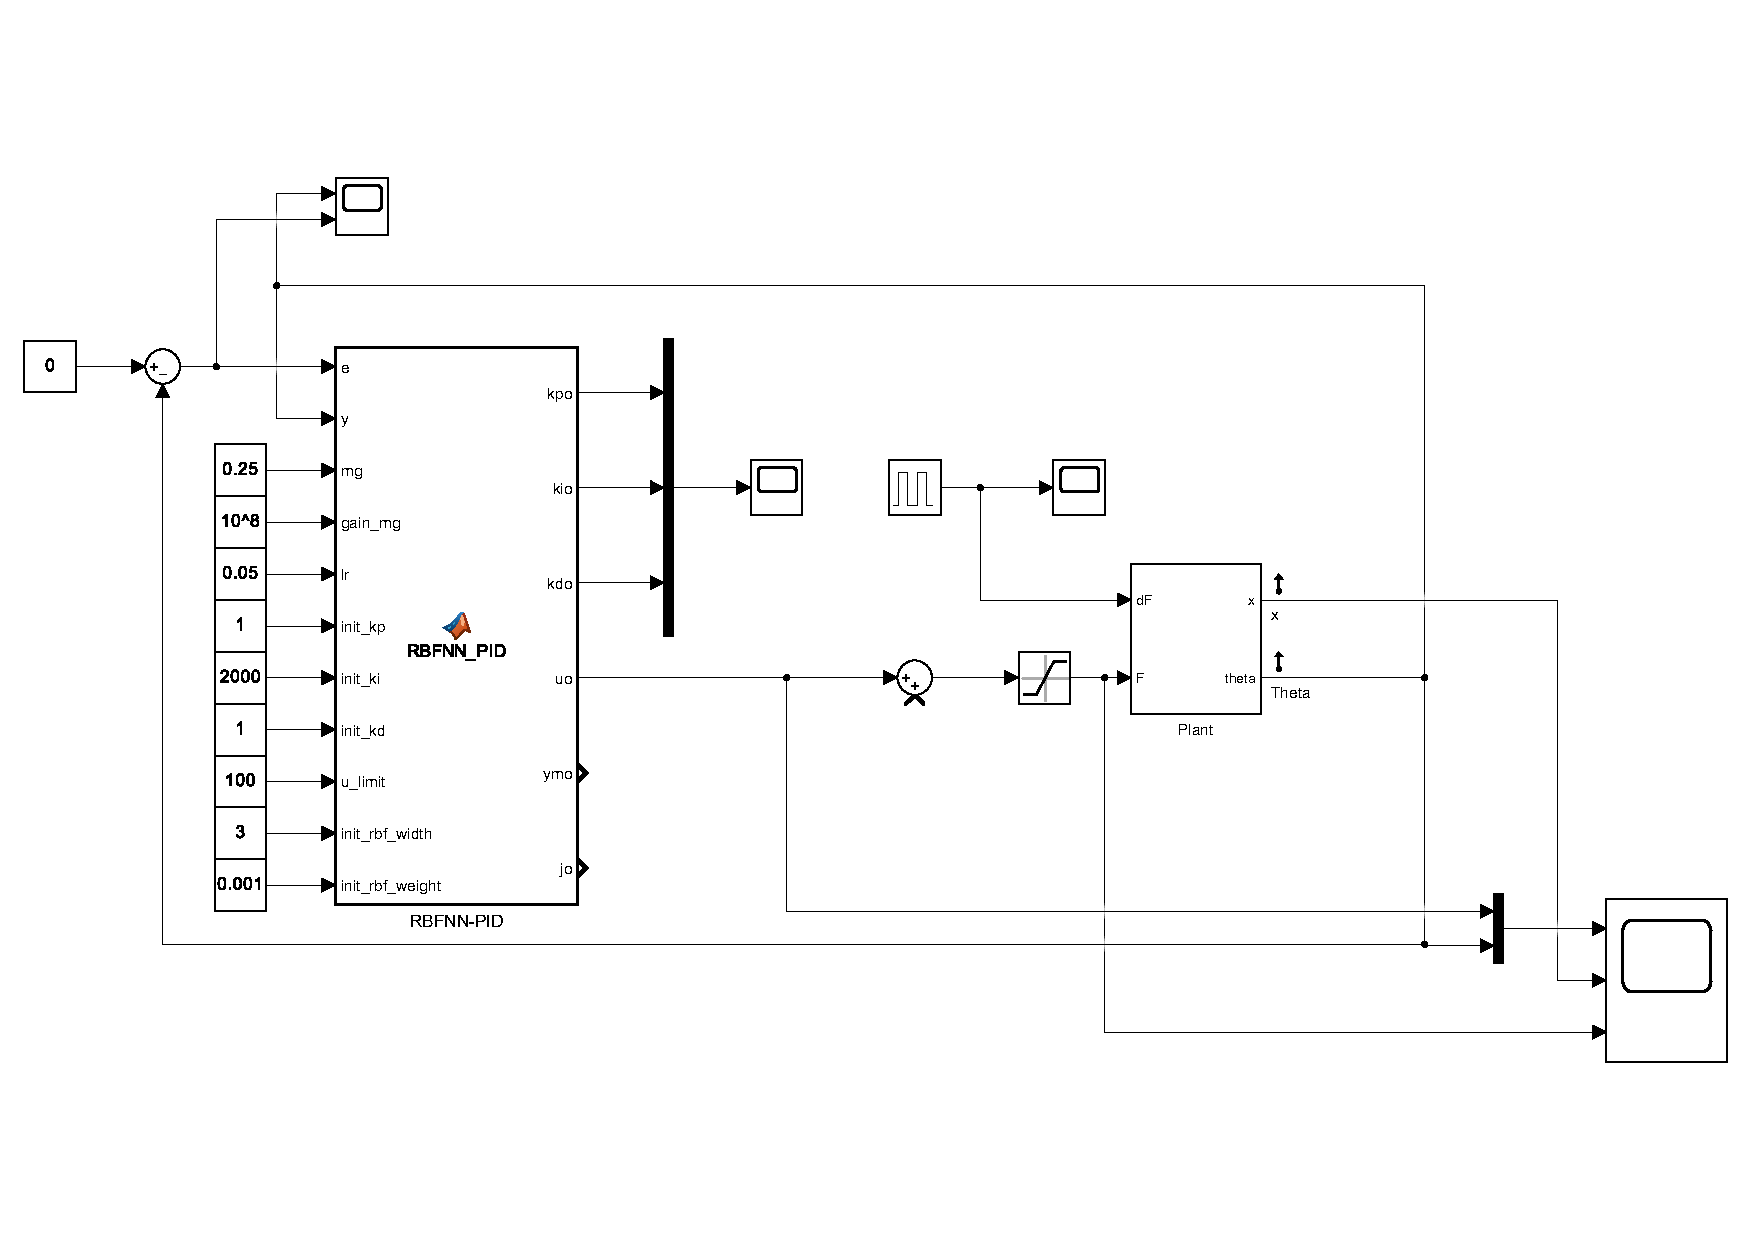
\includegraphics[width=\textwidth,trim={0 3cm 0 3cm},clip]{figures/upper.pdf}
    \caption{Simulink 다이어그램}
    \label{fig:simulink_diagram}
\end{figure}
%
그림 \ref{fig:simulink_diagram}은 2장과 3장에서의 제어기와 신경망, 그리고 Simulink Multibody를 이용해 구현한 이동식 도립 진자의 물리 시뮬레이터를 나타냅니다. 제어기와 신경망을 통합한 RBFNN-PID 블럭과 같을 확인하기 위한 Scope 블럭, 그리고 Plant 블럭과 해당 블럭의 dF 포트의 외란을 모사하기 위한 펄스 출력 블럭, F 포트의 제어기 출력을 제한 하기 위한 포화 블럭으로 구성되어 있습니다.  
%
\newcolumntype{C}{>{\centering\arraybackslash}X}
\begin{table}[h!]
\centering
\begin{tabularx}{5cm}{|C|C|}
 \hline
 $\alpha$ & 0.25 \\ 
 \hline
 $\alpha_{g}$ & $10^5$ \\
 \hline
 $\eta$ & 0.05 \\ 
 \hline
 $K_{p}$ & 1 \\ 
 \hline
 $K_{i}$ & 2000 \\ 
 \hline
 $K_{d}$ & 1 \\
 \hline
 $B$ & 3 \\
 \hline
 $W$ & $10^{-3}$ \\
 \hline
\end{tabularx}
\caption{시뮬레이션에 사용된 초기 매개변수}
\end{table}
%
\begin{figure}[H]
    \centering
    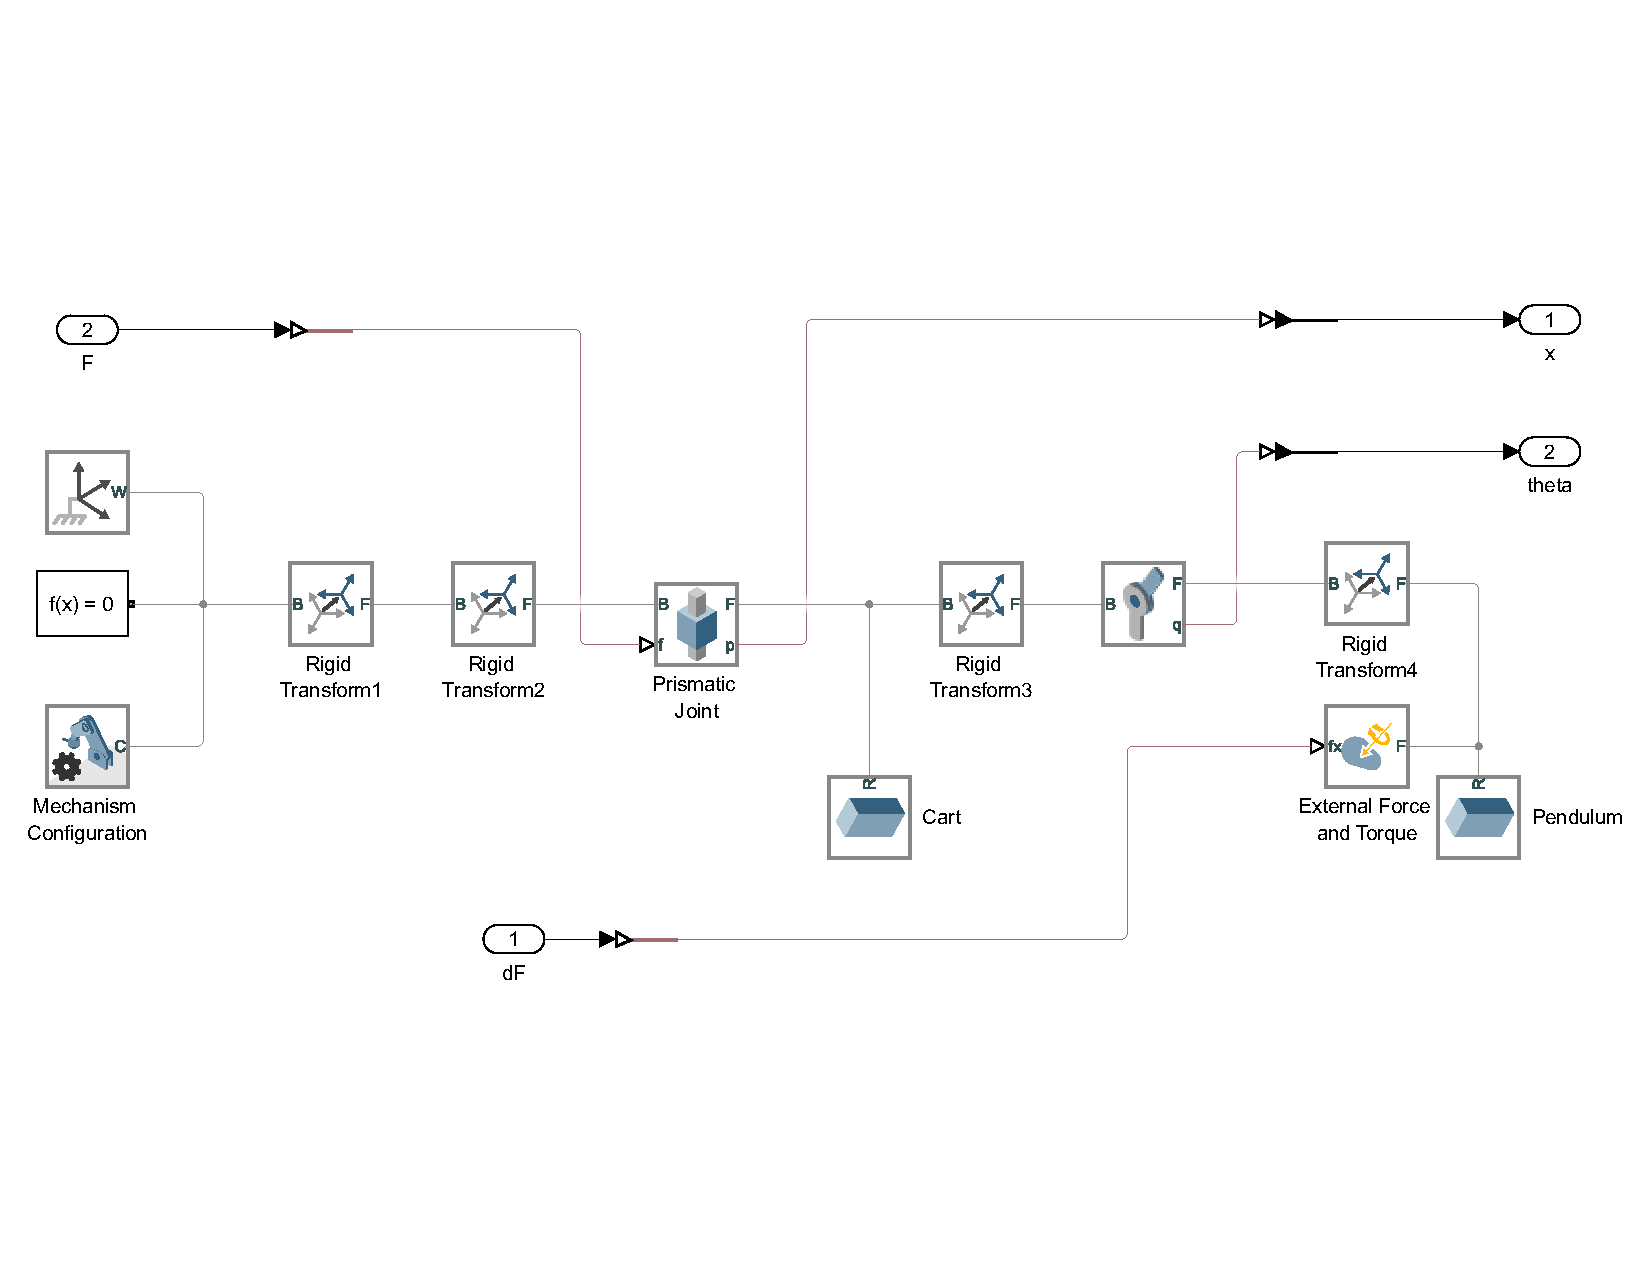
\includegraphics[width=0.8\textwidth,trim={0 3cm 0 3cm},clip]{figures/plant.pdf}
    \caption{Plant Multibody 다이어그램}
    \label{fig:multibody_diagram}
\end{figure}
%
그림 \ref{fig:multibody_diagram}는 그림 \ref{fig:simulink_diagram}의 Plant 블럭의 내부 구조를 나타낸 것입니다. 카트와 진자 및 좌표계 변환 블럭, 경첩 등으로 구성되어 있습니다.
%
\begin{figure}[H]
    \centering
    \begin{tikzpicture}
    \pgfplotsset{set layers}
    \begin{axis}[
        scale only axis,
        xlabel = 시간 (sec),
        ylabel = {$K_{p}$와 $K_{d}$},
        axis y line* = left,
        width = 8cm,
        height = 4cm,
    ]
        \addplot[solid, black] table [col sep=comma, x=time, y=kp]{simulation_data.csv};
        \label{plot_p}
        \addplot[solid, red] table [col sep=comma, x=time, y=kd]{simulation_data.csv};
        \label{plot_d}
    \end{axis}
    \begin{axis}[
        scale only axis,
        ylabel = {$K_{i}$},
        hide x axis,
        axis y line*=right,
        width = 8cm,
        height = 4cm,
        legend style={at={(0.8, 0.5)}},
    ]
        \addlegendimage{/pgfplots/refstyle=plot_p}\addlegendentry{$K_{p}$}
        \addlegendimage{/pgfplots/refstyle=plot_d}\addlegendentry{$K_{d}$}
        \addplot[solid, blue] table [col sep=comma, x=time, y=ki]{simulation_data.csv};
        \addlegendentry{$K_{i}$}
    \end{axis}
    \end{tikzpicture}
    \caption{시간에 따른 이득의 변화}
    \label{fig:gain}
\end{figure}
%
그림 \ref{fig:gain}은 RBF 신경망에 의해 동적으로 조정되는 3가지 이득 계수를 시간에 따라 보여줍니다. 초반 4초까지 시스템의 최적화를 위해 이득이 급격하게 변하다가 그 이후 어느정도 안정을 찾고 수렴하는 것을 관찰할 수 있습니다.
%
\begin{figure}[H] 
    \centering
    \begin{tikzpicture}[yscale=0.7, xscale=0.7]
    \pgfplotsset{set layers}
    \begin{axis}[
        scale only axis,
        xlabel = 시간 (sec),
        axis y line* = left,
        height = 5cm,
    ]
        \addplot[solid, blue] table [col sep=comma, x=time, y=ym]{simulation_data.csv};
        \addlegendentry{$y_{m}$}
        \addplot[solid, red] table [col sep=comma, x=time, y=j]{simulation_data.csv};
        \addlegendentry{$J$}
    \end{axis}
    \end{tikzpicture}
    %\caption{시간에 따른 신경망 출력과\\ 야코비안의 변화}
    %\label{fig:enter-label}   
%\end{figure}
%\begin{figure}[h]
    \centering
    \begin{tikzpicture}[yscale=0.7, xscale=0.7]
    \pgfplotsset{set layers}
    \begin{axis}[
        scale only axis,
        xlabel = 시간 (sec),
        ylabel = {$u$},
        axis y line* = left,
        height = 5cm,
    ]
        \addplot[solid, blue] table [col sep=comma, x=time, y=u]{simulation_data.csv};
        \label{plot_u}
    \end{axis}
    \begin{axis}[
        scale only axis,
        ylabel = {$\theta$},
        hide x axis,
        axis y line*=right,
        height = 5cm,
        legend style={at={(0.9, 1.7)}},
    ]
        \addlegendimage{/pgfplots/refstyle=plot_u}\addlegendentry{$u$}
        \addplot[solid, red] table [col sep=comma, x=time, y=Theta]{simulation_data.csv};
        \addlegendentry{$\theta$}
    \end{axis}
    \end{tikzpicture}
    \captionsetup{justification=centering}
    \caption{\textbf{(좌)} 시간에 따른 신경망 출력과 야코비안의 변화\\ \textbf{(우)} 시간에 따른 제어기 출력과 플랜트 각도의 변화}
    \label{fig:nn-plant}
\end{figure}
%
그림 \ref{fig:nn-plant}의 좌측 그래프는 시간에 따른 신경망의 내부 변수인 \(y_{m}\)과 \(J\)를 나타냅니다. 초기값에서 시작하여 1초 이전에 시스템이 안정화되어 급격히 제어량이 줄어듬을 확인할 수 있습니다. 우측 그래프는 플랜트의 입력(제어기의 출력)과 플랜트의 상태(각도)를 나타냅니다. 플랜트의 각도가 0도 주변에서 안정되게 제어됨을 확인할 수 있습니다. 시뮬레이션이 \(10^{-5}\)초 해상도로 수행됨에 반해 그래프의 데이터는 \(10^{-1}\)초 해상도로 그려졌으므로 어느정도 왜곡이 존재합니다.

% \clearpage